\chapter{Sputtering of Nanowires}

This chapter will investigate the sputtering of nanowires. The experiments were conducted together with Stefan Noack and are partially published in his master thesis \cite{noack_sputter_2014} and in Nano Letters \cite{}.

\section{First results in $Mn$ irradiated $GaAs$}

Introduction by Mn in GaAs (JPhysD)


\section{Simulation results}
\label{sec:simsputering}

A good understanding of the sputtering of nanowires can be gained by looking at MC simulations results performed with \emph{iradina}. From the discussion of the Sigmund sputter model in chapter \ref{sec:ionsolid} a maximum is expected for a certain ion, ion energy and nanowire diameter combination. This can be seen in figure \ref{sputterplot}a \ref{sputterplot}b for the examples of $Xe^+$ and $Ar^+$ ions respectively irradiating a nanowire at an angle of $45^\circ$ to the nanowire. For both irradiations a black line indicates the ion range calculated with SRIM and projected on to $45^\circ$. The maximum of the sputtering correlates very well with the ion range. 

The ion range is an even better predictor for maximum sputtering than the first approximation made with the Sigmund sputtering model, which would predict that the sputtering is maximal where the depth of the damage and the radius coincide. For the Gaussian ellipsoid approximation, a Gaussian peak is fitted to the recoil profile for both ions in $Si$ \cite{bobes_ion_2012}. The so found mean damage depth is constantly around $0,7\times$ as less than ion range for the whole energy range investigated here. Thereby it lies on the geometric mean of the nanowire radius and diameter. The reason for the inaccuracy of the Sigmund model can be found in the asymmetry of the damage profile, which has a shoulder on the lower irradiation depth which is not approximated well by the Gaussian profile. This shoulder pushes the maximum overlap between the real damage and a given cylinder surface to larger energies.


The sputter yield is plotted as a function of the nanowire diameter and the ion energy. The difference in sputter yields between $Xe^+$ and $Ar^+$ 

Note that the color profile is not identical as sputtering is about a factor of $2\times$ larger for the denser collision cascedes 
 The ion range calculated using SRIM is plotted as a black curve.



 
Xe, Ar in Si NW: Energy and Diameter dependent SY

\section{$Si$ nanowire sputtering by $Ar^+$ irradiation}
\label{sec:sisputtering}

The experimental verification of this diameter dependent maximum in sputtering was investigated on etched $Si$-nanowire arrays. Figure \ref{Sisputtering} shows the sputter yield for nanowires plotted vs. their diameter. 

The nanowires were irradiated rotated at an angle of $45^\circ$ to the ion beam of $Ar^+$ at $100$ and $300\,keV$. To prevent defect induced density changes and the $Si$ from amorphizing, the irradiation stage was heated to $300^\circ$, as at this temperature the amorphization threshold becomes arbitrarily high \cite{pelaz_ion-beam-induced_2004}. After a fluence of $10^{16}\,cm^{-2}$ the change in diameter was close to the resolution limit of the SEM, therefore only the data for the following two irradiation steps of $2\cdot 10^{16}\,cm^{-2}$ ions is shown.


\section{Redeposition}
\label{sec:redeposition}

While irradiating a nanowire which is standing perpendicular on a substrate as shown in \ref{} material will also be sputtered from the substrate. Some of the sputtered material from the substrate will be redeposited on the nanowire, so that the observable sputter yield will be lower than the actual sputtering. Consider the situation shown in figure \ref{redeposit}. An ion hits the substrate at point A. A possible path of a sputtered atom is indicated by the red line to a point on the nanowire, redepositing the substrate atom on the nanowire. 

\begin{SCfigure}
	\centering
		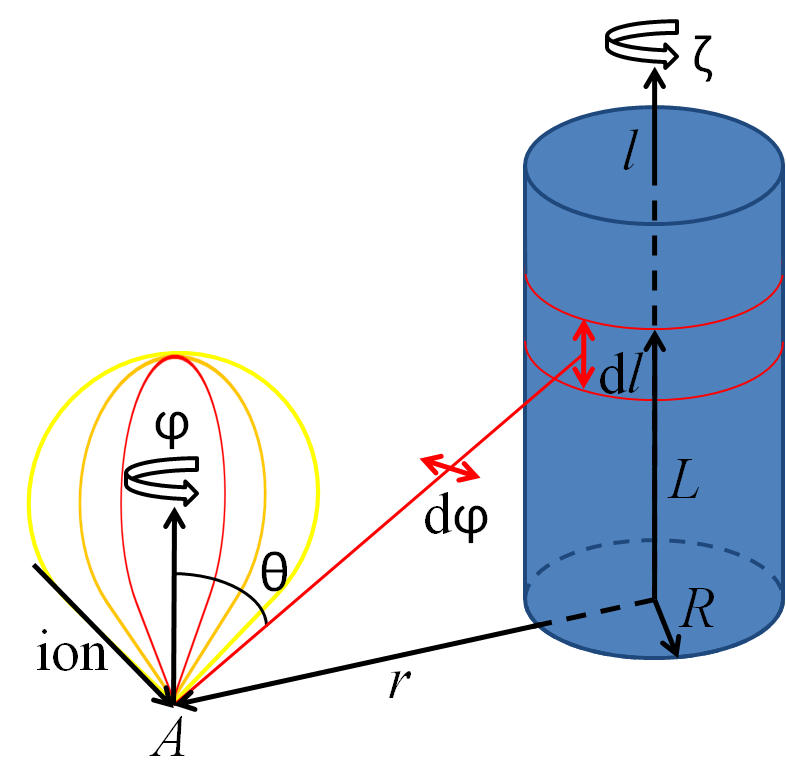
\includegraphics[width=.48\textwidth]{images/redeposit.jpg}
	\caption{Illustration of the redeposition of sputtered material from the substrate point A onto the nanowire with radius R at a height L. Since the wire is rotated around its axis $\zeta$ and the whole substrate is irradiated, a rotationally symmetric angle distribution for the sputtered atoms can be chosen.} 
	\label{redeposit}
\end{SCfigure}

The following calculation will estimate how large the redeposition is, by first calculating the probability of a sputtered atom to hit the nanowire $P$:

\begin{equation}
\label{prob1}
P = \int_0^{2\pi} \! \,\int_0^{\pi/2} \!\! H(\theta,\varphi,r,R,L) \, \tilde{SY}(\theta,\varphi) \,cos(\theta)\,\mathrm{d}\theta \, \mathrm{d}\varphi.
\end{equation}

Where $H(\theta,\varphi,r,R,L)$ is the probability distribution of hitting the nanowire. It is $1/(4\pi)$ if the trajectory along $\theta$ and $\varphi$ from $r$ hits the nanowire with length $L$ and radius $R$, and zero otherwise. For irradiation at an angle, the angle distribution of the sputter yield $\tilde{SY}(\theta,\varphi)$ is expected to have a preferential direction along the ion beam \cite{verdeil_angular_2008}. However, the effective distribution becomes rotationally symmetric (independent of the angle $\varphi$) if one neglects the shadowing of the ion beam on the substrate, as all points around the wire are irradiated and the wire is rotated around its axis (angle $\zeta$). This means that a rotationally symmetric angle distribution $\tilde{SY}(\theta)$ of the sputtered atoms from the substrate can be used, as indicated by the yellow, orange and red bulbs. A $cos^\kappa(\theta)$ distribution is chosen, as it forms flattened angle distributions for $\kappa < 1$, which can emulate the rotation of a slanted angle distribution: 

\begin{equation}
\tilde{SY}(\theta) = \frac{SY \cdot cos^\kappa(\theta)}{\int_0^{2\pi} \! \mathrm{d}\tilde\varphi \,\int_0^{\pi/2} \! cos^\kappa(\tilde\theta) cos(\tilde\theta)\,  \mathrm{d}\tilde\theta} \, = SY /c(\kappa) \cdot cos^\kappa(\theta) ,
\end{equation}

where the denominator $c(\kappa)$ normalizes the angle distribution function $cos^\kappa(\theta)$ and $SY$ is the total sputter yield from the surface. The parametrization of $H(\theta,\varphi,r,R,L)$ in $\varphi$ is straightforward, as the integration bounds for $\varphi$ are $[-\gamma, \gamma]$ with $\gamma = arcsin(R/r)$ the angle between $r$ and the tangent to the nanowire in figure \ref{anglesredepo} a). To solve the integration over $\theta$ it is useful to express the distance $q$ from the impact point to the base of the nanowire can be expressed as a function of $\rho = R/r, r$ and $\varphi$:

\begin{equation}
q(\rho,r,\varphi) = r\cdot \sqrt{1 + \rho^2 - 2sin^2(\varphi) - \sqrt{cos^2(\varphi)(cos(2\varphi) - 1 + 2\rho^2)}},
\end{equation}

\begin{figure}
	\centering
		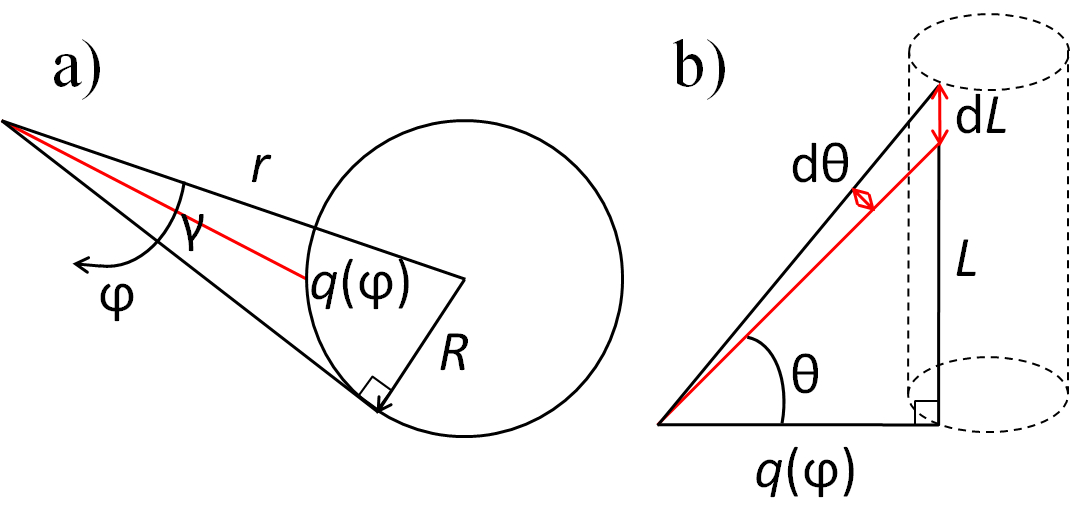
\includegraphics[width=.6\textwidth]{images/anglesredeposition.jpg}
	\caption{a) On the substrate surface $R$ is the radius of the nanowire, $r$ the distance from the point of impact A to the center of the wire, $q(\phi)$ the distance to the wires surface at the base of the wire. The angle between $r$ and the tangent to the nanowire circumference is $\gamma$. b) Side on view with $\theta$ the angle to the substrate normal of the trajectory to hit the wire at $L$.} 
	\label{anglesredepo}
\end{figure} 

to be able to substitute the integration over $\theta$ by an integration over the length of the nanowire $l$. The substitution can be found looking at figure \ref{anglesredepo} b):

\begin{align*}
\mathrm{d}\theta &= \frac{sin(\theta)}{\sqrt{L^2 + q^2}}\,\mathrm{d}L\\
\theta &= arctan(L/q)
\end{align*}

Inserting into equation \ref{prob1} and simplifying yields:

\begin{equation}
\label{prob2}
P = \frac{2\,SY}{c} \int_0^{\gamma} \! \int_{L_1}^{L_2} \!  \frac{l\,q^{\kappa+1}}{(l^2 + q^2)^{(\kappa + 3)/2}} \,\mathrm{d}l \, \mathrm{d}\varphi.
\end{equation}

With $l^*=L_1-L_2$ the area hit on the nanowire is now $\pi \, R \, l^*$, positioned at the height $L= (L_1+L_2)/2$ as indicated between the two red lines in figure \ref{redeposit}. Integrating the probability $P$ to hit the nanowire at each substrate position over the whole substrate area and normalizing it to the area of the nanowire which is hit yields the number of atoms $N$ hitting the nanowire per fluence $\Phi$:

\begin{equation}
\label{prob2}
N/\Phi = \frac{2\,SY}{c \pi Rl^*} \int_0^{2\pi}\! \mathrm{d}\zeta \int_R^{\infty} \!
\int_0^{\gamma} \! \int_{L_1}^{L_2} \! r \frac{l\,q^{\kappa+1}}{(l^2 + q^2)^{(\kappa + 3)/2}}\,\,\mathrm{d}l \, \mathrm{d}\varphi\,\mathrm{d}r \, .
\end{equation}

The integration can be solved numerically using \TODO{numerical tools}. Perhaps counter-intuitively, the result is independent of the nanowire radius $R$ and the height at $L$ at which the deposition is calculated. However, this can be made plausible by looking at figure \ref{anglesredepo}. There is no characteristic radius $R_c$ which would change any of the geometric relations in \ref{anglesredepo}a. Since the integration is over all the $r > R$ and necessarily always starts at $P(R) =1/2$ and goes to $P(r\rightarrow \infty) =0$, its result is independent of $R$. For $L$ it can be argued in figures \ref{anglesredepo}b or \ref{redeposit} that for a fixed $\theta$, $\mathrm{d}L \propto 1/r$ scales as the inverse of the area $\mathrm{d}A \propto r$ of the annulus radiating towards the nanowire under that angle. Therefore the redeposition is constant along the whole nanowire length. 

 
